%% AMS-LaTeX Created with the Wolfram Language : www.wolfram.com

\documentclass{article}
\usepackage{amsmath, amssymb, graphics, setspace}

\newcommand{\mathsym}[1]{{}}
\newcommand{\unicode}[1]{{}}

\newcounter{mathematicapage}
\begin{document}

\begin{doublespace}
\noindent\(\pmb{\text{l1}=\{2299,3920,5850,8275,10602,10982,10146,7958\}}\)
\end{doublespace}

\begin{doublespace}
\noindent\(\{2299,3920,5850,8275,10602,10982,10146,7958\}\)
\end{doublespace}

\begin{doublespace}
\noindent\(\pmb{\text{func1}=\text{Table}[\{6.5+0.1i,\text{l1}[[i]]\},\{i,1,8\}]}\)
\end{doublespace}

\begin{doublespace}
\noindent\(\{\{6.6,2299\},\{6.7,3920\},\{6.8,5850\},\{6.9,8275\},\{7.,10602\},\{7.1,10982\},\{7.2,10146\},\{7.3,7958\}\}\)
\end{doublespace}

\begin{doublespace}
\noindent\(\pmb{\text{TableForm}[\{\{\text{{``}$\unicode{9608}\unicode{503c}$/V{''}},6.6,6.7,6.8,6.9,7.,7.1,7.2,7.3\},}\\
\pmb{\{\text{{``}$\unicode{8ba1}\unicode{6570}${''}},2299,3920,5850,8275,10602,10982,10146,7958\}\}]}\)
\end{doublespace}

\begin{doublespace}
\noindent\(\begin{array}{lllllllll}
 \text{$\unicode{9608}\unicode{503c}$/V} & 6.6 & 6.7 & 6.8 & 6.9 & 7. & 7.1 & 7.2 & 7.3 \\
 \unicode{8ba1}\unicode{6570} & 2299 & 3920 & 5850 & 8275 & 10602 & 10982 & 10146 & 7958 \\
\end{array}\)
\end{doublespace}

\begin{doublespace}
\noindent\(\pmb{\text{Show}[\text{ListPlot}[\text{func1}],\text{Plot}[\text{Interpolation}[\text{func1},\text{Method}\text{-$>$}\text{{``}Spline{''}}][x],\{x,6.5,7.5\}],}\\
\pmb{\left.\text{PlotRange}\to \text{All},\text{AxesLabel}\to \left\{\texttt{"}U_{\text{th}}\text{/V$\texttt{"}$},\text{{``}count{''}}\right\}\right]}\)
\end{doublespace}

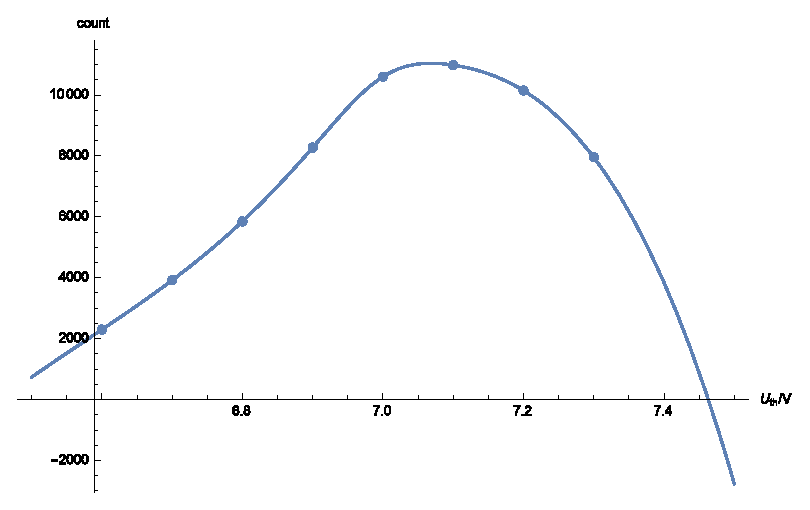
\includegraphics{data_gr1.eps}

\begin{doublespace}
\noindent\(\pmb{\text{Maximize}[\text{Interpolation}[\text{func1},\text{Method}\text{-$>$}\text{{``}Spline{''}}][x],x]}\)
\end{doublespace}

\begin{doublespace}
\noindent\(\{11043.4,\{x\to 7.0682\}\}\)
\end{doublespace}

\begin{doublespace}
\noindent\(\pmb{\text{l2}=}\\
\pmb{\text{Import}[}\\
\pmb{\text{$\texttt{"}$F:$\backslash \backslash $SKF$\backslash \backslash $pku$\backslash \backslash \unicode{5927}\unicode{4e09}\unicode{4e0a}\backslash
\backslash \unicode{8fd1}\unicode{4ee3}\unicode{7269}\unicode{7406}\unicode{5b9e}\unicode{9a8c}\unicode{2160}\backslash \backslash $NaI(Tl)$\unicode{95ea}\unicode{70c1}\unicode{8c31}\unicode{4eea}\unicode{6d4b}\unicode{5b9a}\gamma
\unicode{5c04}\unicode{7ebf}\unicode{80fd}\unicode{8c31}\backslash \backslash $skf$\backslash \backslash $cs-}}\\
\pmb{\text{spectrum-data.txt$\texttt{"}$},\text{{``}list{''}}]}\)
\end{doublespace}

\begin{doublespace}
\noindent\(\{93,124,341,356,1548,3438,5261,7764,10125,11072,9539,7221,5150,3370,1964,1034,464,311,272,319,313,304,390,435,524,570,793,1019,1347,1570,1831,2129,2299,2411,2361,2318,2321,2400,2245,2235,2201,2300,2182,2211,2291,2315,2310,2346,2438,2405,2477,2548,2705,2889,2909,3119,3301,3517,3541,3267,2790,2547,2422,2356,2412,2413,2317,2351,2323,2369,2447,2601,2453,2430,2438\}\)
\end{doublespace}

\begin{doublespace}
\noindent\(\pmb{\text{func2}=\text{Table}[\{8.1-0.1i,\text{l2}[[i]]\},\{i,1,75\}]}\)
\end{doublespace}

\begin{doublespace}
\noindent\(\{\{8.,93\},\{7.9,124\},\{7.8,341\},\{7.7,356\},\{7.6,1548\},\{7.5,3438\},\{7.4,5261\},\{7.3,7764\},\{7.2,10125\},\{7.1,11072\},\{7.,9539\},\{6.9,7221\},\{6.8,5150\},\{6.7,3370\},\{6.6,1964\},\{6.5,1034\},\{6.4,464\},\{6.3,311\},\{6.2,272\},\{6.1,319\},\{6.,313\},\{5.9,304\},\{5.8,390\},\{5.7,435\},\{5.6,524\},\{5.5,570\},\{5.4,793\},\{5.3,1019\},\{5.2,1347\},\{5.1,1570\},\{5.,1831\},\{4.9,2129\},\{4.8,2299\},\{4.7,2411\},\{4.6,2361\},\{4.5,2318\},\{4.4,2321\},\{4.3,2400\},\{4.2,2245\},\{4.1,2235\},\{4.,2201\},\{3.9,2300\},\{3.8,2182\},\{3.7,2211\},\{3.6,2291\},\{3.5,2315\},\{3.4,2310\},\{3.3,2346\},\{3.2,2438\},\{3.1,2405\},\{3.,2477\},\{2.9,2548\},\{2.8,2705\},\{2.7,2889\},\{2.6,2909\},\{2.5,3119\},\{2.4,3301\},\{2.3,3517\},\{2.2,3541\},\{2.1,3267\},\{2.,2790\},\{1.9,2547\},\{1.8,2422\},\{1.7,2356\},\{1.6,2412\},\{1.5,2413\},\{1.4,2317\},\{1.3,2351\},\{1.2,2323\},\{1.1,2369\},\{1.,2447\},\{0.9,2601\},\{0.8,2453\},\{0.7,2430\},\{0.6,2438\}\}\)
\end{doublespace}

\begin{doublespace}
\noindent\(\pmb{\text{Show}[\text{ListPlot}[\text{func2}],\text{Plot}[\text{Interpolation}[\text{func2},\text{Method}\text{-$>$}\text{{``}Spline{''}}][x],}\\
\pmb{\left.\{x,0.6,8\},\text{PlotRange}\to \text{Full}],\text{PlotRange}\to \text{All},\text{AxesLabel}\to \left\{\texttt{"}U_{\text{th}}\text{/V$\texttt{"}$},\text{{``}count{''}}\right\}\right]}\)
\end{doublespace}

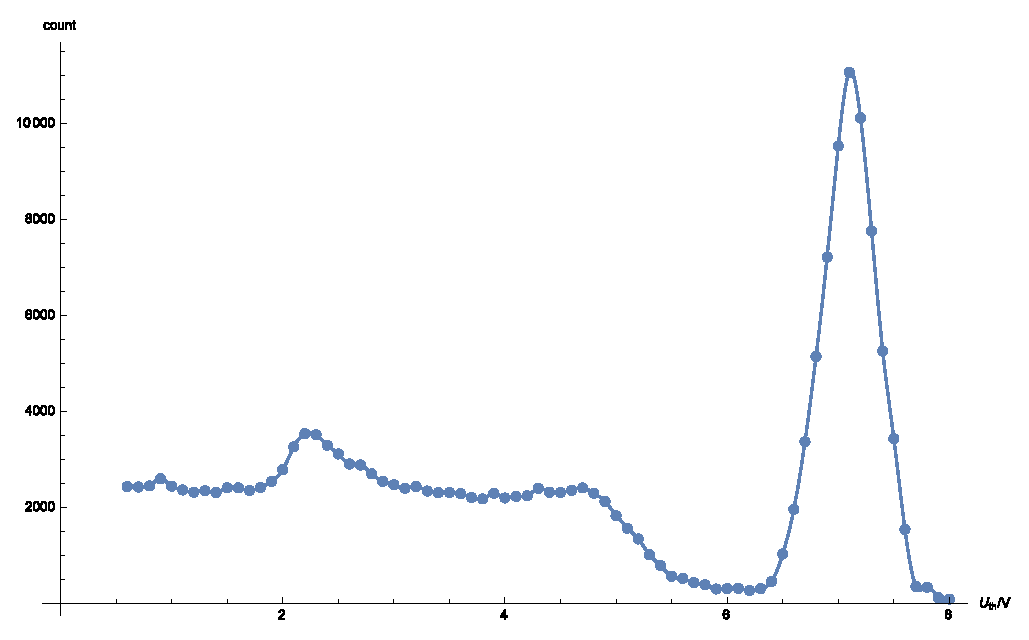
\includegraphics{data_gr2.eps}

\begin{doublespace}
\noindent\(\pmb{\text{Flatten}[}\\
\pmb{\text{Table}[\text{Transpose}[\text{Table}[\{\text{SetAccuracy}[8.1-0.1i,2],\text{l2}[[i]]\},\{i,10j+1,10j+10\}]\text{//}}\\
\pmb{\left.\left.\text{Prepend}\left[\left\{\texttt{"}U_{\text{th}}\text{/V$\texttt{"}$},\text{{``}count{''}}\right\}\right]\right],\{j,0,6\}\right]\text{//}}\\
\pmb{\text{Append}[\text{Transpose}[\text{Table}[\{\text{SetAccuracy}[8.1-0.1i,2],\text{l2}[[i]]\},\{i,71,75\}]\text{//}}\\
\pmb{\left.\left.\left.\text{Prepend}\left[\left\{\texttt{"}U_{\text{th}}\text{/V$\texttt{"}$},\text{{``}count{''}}\right\}\right]\right]\right],1\right]\text{//}\text{TableForm}}\)
\end{doublespace}

\begin{doublespace}
\noindent\(\begin{array}{lllllllllll}
 U_{\text{th}}\text{/V} & 8.0 & 7.9 & 7.8 & 7.7 & 7.6 & 7.5 & 7.4 & 7.3 & 7.2 & 7.1 \\
 \text{count} & 93 & 124 & 341 & 356 & 1548 & 3438 & 5261 & 7764 & 10125 & 11072 \\
 U_{\text{th}}\text{/V} & 7.0 & 6.9 & 6.8 & 6.7 & 6.6 & 6.5 & 6.4 & 6.3 & 6.2 & 6.1 \\
 \text{count} & 9539 & 7221 & 5150 & 3370 & 1964 & 1034 & 464 & 311 & 272 & 319 \\
 U_{\text{th}}\text{/V} & 6.0 & 5.9 & 5.8 & 5.7 & 5.6 & 5.5 & 5.4 & 5.3 & 5.2 & 5.1 \\
 \text{count} & 313 & 304 & 390 & 435 & 524 & 570 & 793 & 1019 & 1347 & 1570 \\
 U_{\text{th}}\text{/V} & 5.0 & 4.9 & 4.8 & 4.7 & 4.6 & 4.5 & 4.4 & 4.3 & 4.2 & 4.1 \\
 \text{count} & 1831 & 2129 & 2299 & 2411 & 2361 & 2318 & 2321 & 2400 & 2245 & 2235 \\
 U_{\text{th}}\text{/V} & 4.0 & 3.9 & 3.8 & 3.7 & 3.6 & 3.5 & 3.4 & 3.3 & 3.2 & 3.1 \\
 \text{count} & 2201 & 2300 & 2182 & 2211 & 2291 & 2315 & 2310 & 2346 & 2438 & 2405 \\
 U_{\text{th}}\text{/V} & 3.0 & 2.9 & 2.8 & 2.7 & 2.6 & 2.5 & 2.4 & 2.3 & 2.2 & 2.1 \\
 \text{count} & 2477 & 2548 & 2705 & 2889 & 2909 & 3119 & 3301 & 3517 & 3541 & 3267 \\
 U_{\text{th}}\text{/V} & 2.0 & 1.9 & 1.8 & 1.7 & 1.6 & 1.5 & 1.4 & 1.3 & 1.2 & 1.1 \\
 \text{count} & 2790 & 2547 & 2422 & 2356 & 2412 & 2413 & 2317 & 2351 & 2323 & 2369 \\
 U_{\text{th}}\text{/V} & 1. & 0.9 & 0.8 & 0.7 & 0.6 & \text{} & \text{} & \text{} & \text{} & \text{} \\
 \text{count} & 2447 & 2601 & 2453 & 2430 & 2438 & \text{} & \text{} & \text{} & \text{} & \text{} \\
\end{array}\)
\end{doublespace}

\begin{doublespace}
\noindent\(\pmb{\text{Maximize}[\{\text{Interpolation}[\text{func2},\text{Method}\text{-$>$}\text{{``}Spline{''}}][x],x\geq 6\&\&x\leq 8\},x]}\)
\end{doublespace}

\begin{doublespace}
\noindent\(\{11092.,\{x\to 7.11128\}\}\)
\end{doublespace}

\begin{doublespace}
\noindent\(\pmb{\text{func20}=\text{Interpolation}[\text{func2},\text{Method}\text{-$>$}\text{{``}Spline{''}}]}\)
\end{doublespace}

\begin{doublespace}
\noindent\(\text{InterpolatingFunction}[]\)
\end{doublespace}

\begin{doublespace}
\noindent\(\pmb{\text{MaxValue}[\{\text{func20}[x],x\geq 6\&\&x\leq 8\},x]/2}\)
\end{doublespace}

\begin{doublespace}
\noindent\(5545.99\)
\end{doublespace}

\begin{doublespace}
\noindent\(\pmb{\text{FindRoot}[\text{func20}[x]==5545.99,\{x,7.0\}]}\)
\end{doublespace}

\begin{doublespace}
\noindent\(\{x\to 6.82035\}\)
\end{doublespace}

\begin{doublespace}
\noindent\(\pmb{\text{l3}=}\\
\pmb{\text{Import}[}\\
\pmb{\text{$\texttt{"}$F:$\backslash \backslash $SKF$\backslash \backslash $pku$\backslash \backslash \unicode{5927}\unicode{4e09}\unicode{4e0a}\backslash
\backslash \unicode{8fd1}\unicode{4ee3}\unicode{7269}\unicode{7406}\unicode{5b9e}\unicode{9a8c}\unicode{2160}\backslash \backslash $NaI(Tl)$\unicode{95ea}\unicode{70c1}\unicode{8c31}\unicode{4eea}\unicode{6d4b}\unicode{5b9a}\gamma
\unicode{5c04}\unicode{7ebf}\unicode{80fd}\unicode{8c31}\backslash \backslash $skf$\backslash \backslash $cs-co-}}\\
\pmb{\text{peak-data.txt$\texttt{"}$},\text{{``}list{''}}]}\)
\end{doublespace}

\begin{doublespace}
\noindent\(\{4658,4994,5419,6629,6253,5665,2556,6280,15113,19979,18304,9731,8588,8488,8904,11730,15044,20474,22012,18971,11618,6221,6212,9261,12932,16575,16434,11946,6605\}\)
\end{doublespace}

\begin{doublespace}
\noindent\(\pmb{\text{func3}=}\\
\pmb{\{\{\text{Table}[0.8+0.1i,\{i,0,5\}],\text{Table}[3.3+0.1i,\{i,0,5\}],}\\
\pmb{\text{Table}[5.8+0.1i,\{i,0,16\}]\}\text{//}\text{Flatten},\text{l3}\}\text{//}\text{Transpose}}\)
\end{doublespace}

\begin{doublespace}
\noindent\(\{\{0.8,4658\},\{0.9,4994\},\{1.,5419\},\{1.1,6629\},\{1.2,6253\},\{1.3,5665\},\{3.3,2556\},\{3.4,6280\},\{3.5,15113\},\{3.6,19979\},\{3.7,18304\},\{3.8,9731\},\{5.8,8588\},\{5.9,8488\},\{6.,8904\},\{6.1,11730\},\{6.2,15044\},\{6.3,20474\},\{6.4,22012\},\{6.5,18971\},\{6.6,11618\},\{6.7,6221\},\{6.8,6212\},\{6.9,9261\},\{7.,12932\},\{7.1,16575\},\{7.2,16434\},\{7.3,11946\},\{7.4,6605\}\}\)
\end{doublespace}

\begin{doublespace}
\noindent\(\pmb{\text{Grid}\left[\text{Flatten}\left[\left\{\text{func3}[[1\text{;;}10]]\text{//}\text{Prepend}\left[\left\{\texttt{"}U_{\text{th}}\text{/V$\texttt{"}$},\text{{``}count{''}}\right\}\right]\text{//}\text{Transpose},\right.\right.\right.}\\
\pmb{\text{func3}[[11\text{;;}20]]\text{//}\text{Prepend}\left[\left\{\texttt{"}U_{\text{th}}\text{/V$\texttt{"}$},\text{{``}count{''}}\right\}\right]\text{//}\text{Transpose},}\\
\pmb{\left.\left.\left.\text{func3}[[21\text{;;}29]]\text{//}\text{Prepend}\left[\left\{\texttt{"}U_{\text{th}}\text{/V$\texttt{"}$},\text{{``}count{''}}\right\}\right]\text{//}\text{Transpose}\right\},1\right],\text{Frame}\text{-$>$}\text{All}\right]}\)
\end{doublespace}

\begin{doublespace}
\noindent\(\begin{array}{ccccccccccc}
 U_{\text{th}}\text{/V} & 0.8 & 0.9 & 1. & 1.1 & 1.2 & 1.3 & 3.3 & 3.4 & 3.5 & 3.6 \\
 \text{count} & 4658 & 4994 & 5419 & 6629 & 6253 & 5665 & 2556 & 6280 & 15113 & 19979 \\
 U_{\text{th}}\text{/V} & 3.7 & 3.8 & 5.8 & 5.9 & 6. & 6.1 & 6.2 & 6.3 & 6.4 & 6.5 \\
 \text{count} & 18304 & 9731 & 8588 & 8488 & 8904 & 11730 & 15044 & 20474 & 22012 & 18971 \\
 U_{\text{th}}\text{/V} & 6.6 & 6.7 & 6.8 & 6.9 & 7. & 7.1 & 7.2 & 7.3 & 7.4 & \text{} \\
 \text{count} & 11618 & 6221 & 6212 & 9261 & 12932 & 16575 & 16434 & 11946 & 6605 & \text{} \\
\end{array}\)
\end{doublespace}

\begin{doublespace}
\noindent\(\pmb{\text{l4}=\{\{1.1,0.184\},\{3.6,0.662\},\{6.4,1.17\},\{7.1,1.33\}\}}\)
\end{doublespace}

\begin{doublespace}
\noindent\(\{\{1.1,0.184\},\{3.6,0.662\},\{6.4,1.17\},\{7.1,1.33\}\}\)
\end{doublespace}

\begin{doublespace}
\noindent\(\pmb{\text{LinearModelFit}[\text{l4},x,x]}\)
\end{doublespace}

\begin{doublespace}
\noindent\(\text{FittedModel}[]\)
\end{doublespace}

\begin{doublespace}
\noindent\(\pmb{\text{$\%$144}[\text{{``}AdjustedRSquared{''}}]\text{//}\text{Sqrt}}\)
\end{doublespace}

\begin{doublespace}
\noindent\(0.999612\)
\end{doublespace}

\begin{doublespace}
\noindent\(\pmb{\text{Show}[\text{ListPlot}[\text{l4},\text{PlotStyle}\to \text{Red}],\text{Plot}[\text{$\%$144}[x],\{x,1.1,7.1\}],}\\
\pmb{\left.\text{AxesLabel}\to \left\{\texttt{"}U_{\text{th}}\text{/V$\texttt{"}$},\text{{``}E/MeV{''}}\right\}\right]}\)
\end{doublespace}

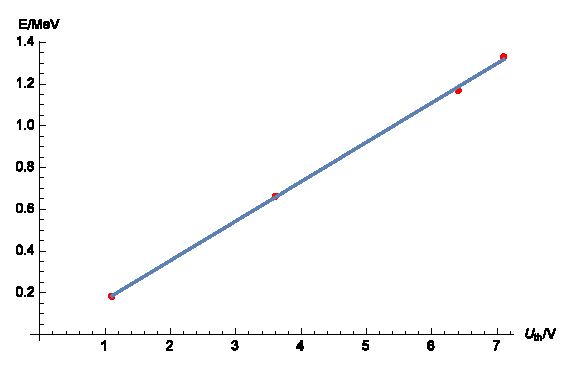
\includegraphics{data_gr3.eps}

\begin{doublespace}
\noindent\(\pmb{\text{l5}=}\\
\pmb{\text{Import}[}\\
\pmb{\text{$\texttt{"}$F:$\backslash \backslash $SKF$\backslash \backslash $pku$\backslash \backslash \unicode{5927}\unicode{4e09}\unicode{4e0a}\backslash
\backslash \unicode{8fd1}\unicode{4ee3}\unicode{7269}\unicode{7406}\unicode{5b9e}\unicode{9a8c}\unicode{2160}\backslash \backslash $NaI(Tl)$\unicode{95ea}\unicode{70c1}\unicode{8c31}\unicode{4eea}\unicode{6d4b}\unicode{5b9a}\gamma
\unicode{5c04}\unicode{7ebf}\unicode{80fd}\unicode{8c31}\backslash \backslash $skf$\backslash \backslash $cs-up.dat}}\\
\pmb{\text{.txt$\texttt{"}$},\text{{``}list{''}}];}\\
\pmb{\text{l6}=}\\
\pmb{\text{Import}[}\\
\pmb{\text{$\texttt{"}$F:$\backslash \backslash $SKF$\backslash \backslash $pku$\backslash \backslash \unicode{5927}\unicode{4e09}\unicode{4e0a}\backslash
\backslash \unicode{8fd1}\unicode{4ee3}\unicode{7269}\unicode{7406}\unicode{5b9e}\unicode{9a8c}\unicode{2160}\backslash \backslash $NaI(Tl)$\unicode{95ea}\unicode{70c1}\unicode{8c31}\unicode{4eea}\unicode{6d4b}\unicode{5b9a}\gamma
\unicode{5c04}\unicode{7ebf}\unicode{80fd}\unicode{8c31}\backslash \backslash $skf$\backslash \backslash $cs-down.}}\\
\pmb{\text{dat.txt$\texttt{"}$},\text{{``}list{''}}];}\\
\pmb{\text{l7}=}\\
\pmb{\text{Import}[}\\
\pmb{\text{$\texttt{"}$F:$\backslash \backslash $SKF$\backslash \backslash $pku$\backslash \backslash \unicode{5927}\unicode{4e09}\unicode{4e0a}\backslash
\backslash \unicode{8fd1}\unicode{4ee3}\unicode{7269}\unicode{7406}\unicode{5b9e}\unicode{9a8c}\unicode{2160}\backslash \backslash $NaI(Tl)$\unicode{95ea}\unicode{70c1}\unicode{8c31}\unicode{4eea}\unicode{6d4b}\unicode{5b9a}\gamma
\unicode{5c04}\unicode{7ebf}\unicode{80fd}\unicode{8c31}\backslash \backslash $skf$\backslash \backslash $co-down.}}\\
\pmb{\text{dat.txt$\texttt{"}$},\text{{``}list{''}}];}\\
\pmb{\text{l8}=}\\
\pmb{\text{Import}[}\\
\pmb{\text{$\texttt{"}$F:$\backslash \backslash $SKF$\backslash \backslash $pku$\backslash \backslash \unicode{5927}\unicode{4e09}\unicode{4e0a}\backslash
\backslash \unicode{8fd1}\unicode{4ee3}\unicode{7269}\unicode{7406}\unicode{5b9e}\unicode{9a8c}\unicode{2160}\backslash \backslash $NaI(Tl)$\unicode{95ea}\unicode{70c1}\unicode{8c31}\unicode{4eea}\unicode{6d4b}\unicode{5b9a}\gamma
\unicode{5c04}\unicode{7ebf}\unicode{80fd}\unicode{8c31}\backslash \backslash $skf$\backslash \backslash $cs-co-}}\\
\pmb{\text{down.dat.txt$\texttt{"}$},\text{{``}list{''}}];}\)
\end{doublespace}

\begin{doublespace}
\noindent\(\pmb{\text{ListPlot}[\text{l5},\text{PlotRange}\to \text{All},\text{AxesLabel}\to \{\text{{``}$\unicode{9053}\unicode{6570}${''}},\text{{``}count{''}}\}]}\)
\end{doublespace}

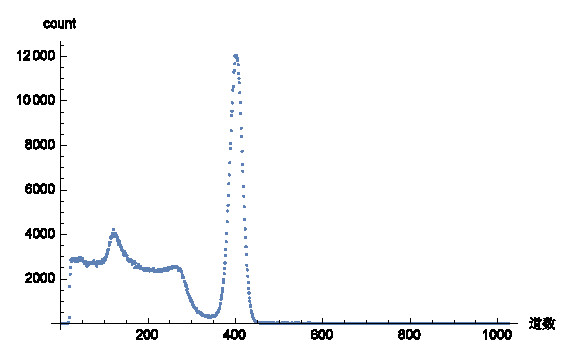
\includegraphics{data_gr4.eps}

\begin{doublespace}
\noindent\(\pmb{\text{ListPlot}[\text{l6},\text{AxesLabel}\to \{\text{{``}$\unicode{9053}\unicode{6570}${''}},\text{{``}count{''}}\}]}\)
\end{doublespace}

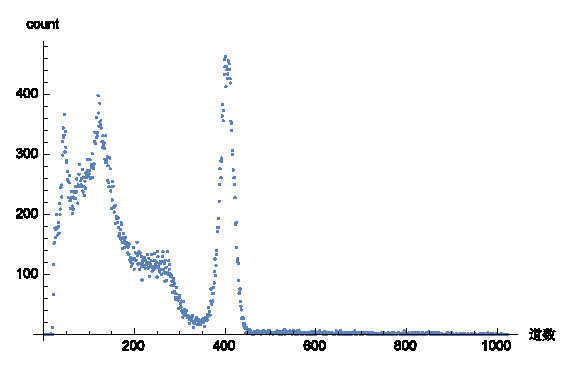
\includegraphics{data_gr5.eps}

\begin{doublespace}
\noindent\(\pmb{\text{ListPlot}[\text{l7},\text{AxesLabel}\to \{\text{{``}$\unicode{9053}\unicode{6570}${''}},\text{{``}count{''}}\}]}\)
\end{doublespace}

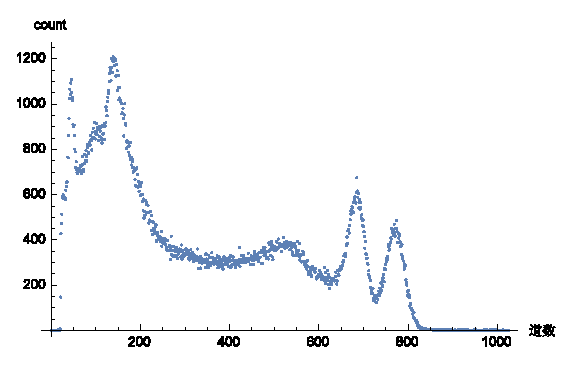
\includegraphics{data_gr6.eps}

\begin{doublespace}
\noindent\(\pmb{\text{ListPlot}[\text{l8},\text{AxesLabel}\to \{\text{{``}$\unicode{9053}\unicode{6570}${''}},\text{{``}count{''}}\}]}\)
\end{doublespace}

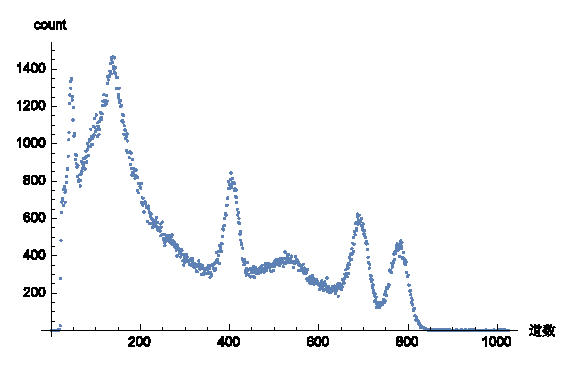
\includegraphics{data_gr7.eps}

\begin{doublespace}
\noindent\(\pmb{\text{ListPlot}[\text{l8}-\text{l7}-\text{l6},\text{AxesLabel}\to \{\text{{``}$\unicode{9053}\unicode{6570}${''}},\text{{``}count{''}}\}]}\)
\end{doublespace}

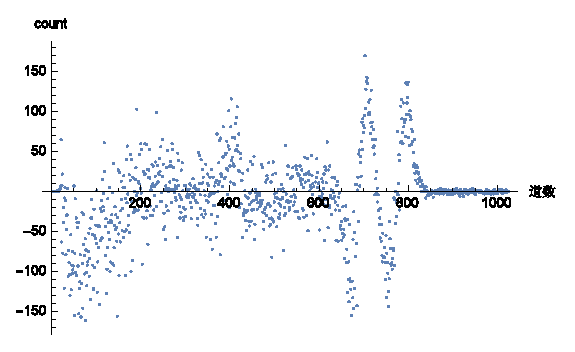
\includegraphics{data_gr8.eps}

\begin{doublespace}
\noindent\(\pmb{\text{l9}=\{\{125,0.184\},\{400,0.662\},\{690,1.17\},\{770,1.33\}\}}\)
\end{doublespace}

\begin{doublespace}
\noindent\(\{\{125,0.184\},\{400,0.662\},\{690,1.17\},\{770,1.33\}\}\)
\end{doublespace}

\begin{doublespace}
\noindent\(\pmb{\text{LinearModelFit}[\text{l9},x,x]}\)
\end{doublespace}

\begin{doublespace}
\noindent\(\text{FittedModel}[]\)
\end{doublespace}

\begin{doublespace}
\noindent\(\pmb{\text{$\%$214}[\text{{``}AdjustedRSquared{''}}]\text{//}\text{Sqrt}}\)
\end{doublespace}

\begin{doublespace}
\noindent\(0.99981\)
\end{doublespace}

\begin{doublespace}
\noindent\(\pmb{\text{Show}[\text{ListPlot}[\text{l9},\text{PlotStyle}\to \text{Red}],\text{Plot}[\text{$\%$214}[x],\{x,125,770\}],}\\
\pmb{\text{AxesLabel}\to \{\text{{``}$\unicode{9053}\unicode{6570}${''}},\text{{``}count{''}}\}]}\)
\end{doublespace}

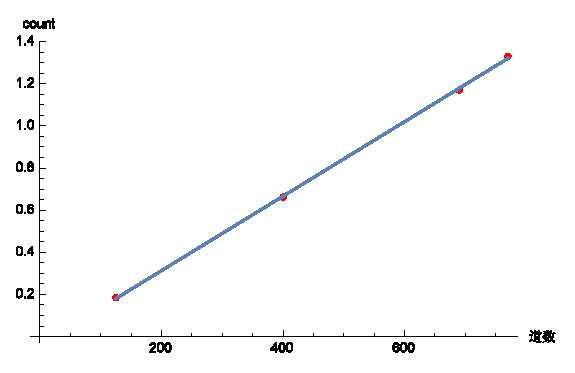
\includegraphics{data_gr9.eps}

\begin{doublespace}
\noindent\(\pmb{\text{l9}/\text{l4}}\)
\end{doublespace}

\begin{doublespace}
\noindent\(\{\{113.636,1.\},\{111.111,1.\},\{107.813,1.\},\{108.451,1.\}\}\)
\end{doublespace}

\end{document}
